\section{Data Generation}

Since the script of \textcite{geronel2023} provides the control torque (\(\mathbf{\tau}_{\eta}\)) related to the state-space (\(\mathbf{x}_s\) ) through dynamic and control equations.
The ANN goal will take \(\mathbf{x}_s\) as the input vector and predict the \(\mathbf{\tau}_{\eta}\) vector as output.
Modifications in the script are minimal the necessary to generate a thousand trajectories in a loop and adding random noise to each one.
The time is a discrete vector with \SI{200}{s} and step 0.01, therefore the time vector has \(1\times 20000\) dimension.

The output vector \(\mathbf{T}\) has \(20000\times 4\) dimension the and the input vector \(\mathbf{X}_s\) has  \(20000\times 12\) dimension, where each line represents specific point in time:
%
\begin{align}
    \mathbf{T} &= \begin{bmatrix}
        U_1 & U_2 & U_3 & U_4 \\
        \vdots       & \vdots       & \vdots       & \vdots  \\
    \end{bmatrix} 
    \label{eq:tau_input} \\
    \setcounter{MaxMatrixCols}{13}
    \mathbf{X}_s &=
    \begin{bmatrix}
        x&y&z&\phi&\theta&\psi&\dot{x}&\dot{y}&\dot{z}&\dot{\phi}&\dot{\theta}&\dot{\psi} \\
        \vdots & \vdots & \vdots & \vdots & \vdots & \vdots & \vdots & \vdots & \vdots & \vdots & \vdots & \vdots 
    \end{bmatrix}
    \label{eq:xs_output}
\end{align}

Circular trajectory was arbitrary selected as shown in~\cref{fig:trajectory}.
\begin{figure}[!htb]
    \centering
    \caption[Trajectory of the UAV]{Trajectory of the UAV. Circular trajectory was chosen and the thousand other ones generated are only variations with noise added.}
    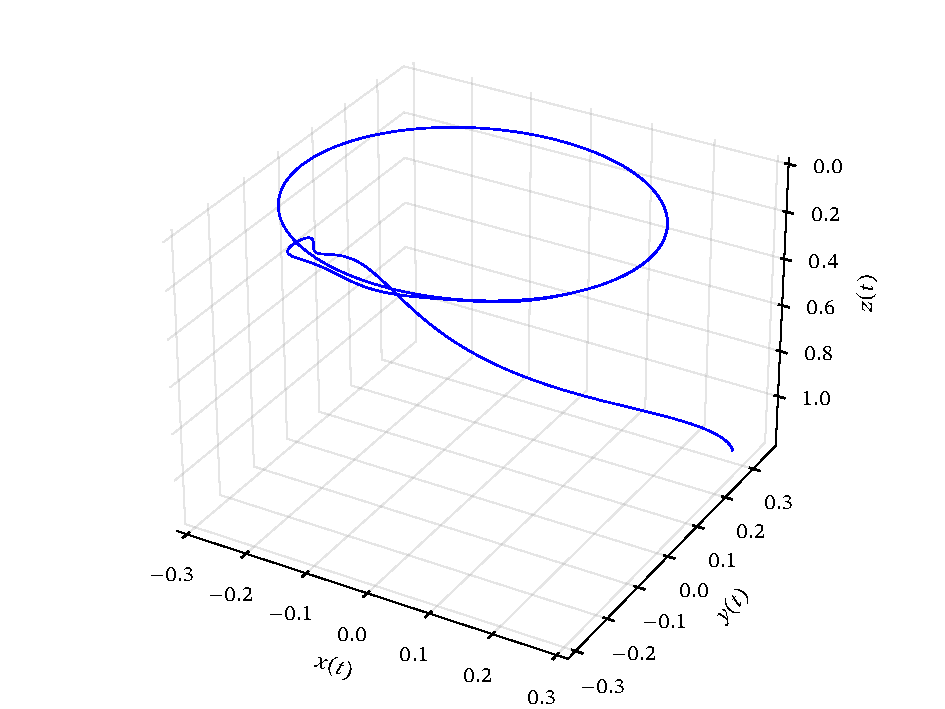
\includegraphics{figures/4results/uav/trajectory.pdf}
    
    \fonte{adapted from \textcite{geronel2023}}
    \label{fig:trajectory}
\end{figure}
Then, it was generated 1000 different trajectories with random noise for each trajectory.
Input and output vector were stored in a MATLAB variable and exported through the \texttt{.mat} extension to be used inside the Python environment using \emph{scipy.io.loadmat} SciPy method.


\section{Algorithm Overview}

The first approach for the ANN is to use the raw data, both for input and output and do the training.
Even though it works, it does not give the proper result, due to the scale for each force and state-space columns.
Therefore, the preprocessing of the data is mandatory to get the best results.
Then, all input and output data were normalized in order to get them all standardized.

The normalization is in L2 form, from the \emph{sklearn.preprocessing.normalize} method, applied in each matrix column.
From the trained ANN, all input data should be normalized and naturally the output also will be normalized.
However, the control forces (output data) can not be normalized to be useful, but there is no ``denormalized'' correspondent matrix to the output data from the ANN.

To solve this problem, a second ANN was created to be able to denormalize the output data.
When preprocessing the data, as the normalization is done, both norms of the input and output data are stored and the second ANN is made from them.
The~\cref{fig:nns_scheme} show how the data and the ANNs are related for the training. 
When the training and the validation is done, the ready-to-use model will perform as shown in the~\cref{fig:full_scheme} scheme.

\begin{figure}[!htb]
    \centering
    \caption[Data and ANN relation]{Data and ANN relation. The training data in the extremes are the ones generated by the white box parametric model.}
    \includesvg[pretex=\footnotesize]{figures/3methodology/nns_scheme.svg}

    \fonte{prepared by the author.}
    \label{fig:nns_scheme}
\end{figure}

\begin{figure}[!htb]
    \centering
    \caption[Model in Production]{Model in production. The scheme shows how the process returns the control forces from the state space.}
    \includesvg[pretex=\footnotesize]{figures/3methodology/full_scheme.svg}

    \fonte{prepared by the author.}
    \label{fig:full_scheme}
\end{figure}

\section{Neural Network Modeling}

The ANN 1 is responsible for, from the normalized state space, to return the normalized control forces.
The problem is considered as a regression problem for both ANNs.
The~\cref{eq:function_training_model_uav} shows the functional form of the ANN 1. Input and output data are all matrices.
%
\begin{subequations}\label{eq:function_training_model_uav}
    \begin{align}
        &f\big(x,y,\ldots,\dot{\theta},\dot{\psi}\big) = \langle U_1, U_2, U_3, U_4 \rangle \\
        &f(\mathbf{X}_s) = \mathbf{T}
    \end{align}
\end{subequations}
%
The  ANN 2 is responsible for, from the raw data, to get the norms from each input and output data of the ANN 1.
The problem is considered as a regression problem.
Input and output data are all vectors.
Both ANNs have similar parameters, being the main difference the input and output layer size.
Characteristics of them are provided in the~\cref{tab:nns_char}.

\begin{table}[!htb]
    \centering
    \footnotesize
    \caption{Parameters of the neural networks and their training}
    \begin{tblr}{
         row{even} = {rosa},
         width=0.8\textwidth,
         colspec={Q[0.5\textwidth,l] Q[0.2\textwidth,r] Q[0.2\textwidth,r]}
    }
    \toprule
    {\bfseries\sffamily Parameters} & {\bfseries\sffamily ANN 1} & {\bfseries\sffamily ANN 2} \\
    \midrule
    Input layer neurons   & 12      & 1       \\
    Output layer neurons  & 4       & 1       \\
    Hidden layers neurons & 128     & 128     \\
    Hidden layers         & 8       & 8       \\
    Activation function   & ReLU    & ReLU    \\
    Loss function         & MSE     & MSE     \\
    Optimizer             & Adam    & Adam    \\
    Batch size            & 1       & 1       \\
    Train/test split      & 0.8/0.2 & 0.8/0.2 \\
    Epochs                & 500     & 500     \\
    \bottomrule
    \end{tblr}
    \label{tab:nns_char}

    \fonte{prepared by the author.}
\end{table}

